% ------------------------------------------------------------------
\renewcommand{\thisweek}{MATH327 Week 4}
\renewcommand{\moddate}{Last modified 21 Feb.~2021}
\setcounter{section}{4}
\setcounter{subsection}{0}
\phantomsection
\addcontentsline{toc}{section}{Week 4: Ideal gases}
\section*{Week 4: Ideal gases}

\subsection{Volume, energy levels, and partition function}
This week we apply the canonical ensemble to investigate non-relativistic, classical, ideal gases.
Using statistical physics we will explore how the large-scale behaviours of such gases emerge from the properties of the particles that compose them.
The three adjectives above specify these properties in the case we consider this week: \\[-24 pt]
\begin{itemize}
  \item \textbf{Classical} systems are those for which we can ignore the effects of quantum mechanics.
        At a technical level, this means we assume we can simultaneously define both the position $(x, y, z)$ and the momentum $\vec p = (p_x, p_y, p_z)$ of each particle with arbitrary precision.
  \item \textbf{Non-relativistic} particles move with speeds small compared to the speed of light, which allows us to ignore small effects due to special relativity.
        The particles are therefore governed by the laws Isaac Newton published all the way back in 1687.
        In particular, the energy of each particle of mass $m$ is
        \begin{equation*}
          E_n = \frac{1}{2m} p_n^2,
        \end{equation*}
        where $p_n^2 = \vec p_n \cdot \vec p_n = (p_x)_n^2 + (p_y)_n^2 + (p_z)_n^2$ is the inner (or `dot') product of the momentum vector for the $n$th particle.
  \item \textbf{Ideal} gases are those whose constituent particles don't interact with each other.
        As a result, the total energy of the gas is simply the sum of the energies of the $N$ individual particles,
        \begin{equation}
          E = \frac{1}{2m} \sum_{i = n}^N p_n^2.
        \end{equation}
\end{itemize}

As usual for the canonical ensemble, we consider the gas to be in thermodynamic equilibrium, and in thermal contact with a large external thermal reservoir with which it can exchange energy but not particles.
To prevent particle exchange, we can specify that the gas is enclosed in a box with volume $V = L^3$.
The thermal reservoir fixes the temperature $T$ of the gas.

The starting point for our analysis is to compute the partition function
\begin{equation*}
  Z = \sum_i e^{-E_i / T}.
\end{equation*}
Here the sum is over all possible micro-states $\om_i$ of the $N$-particle system, which is problematic.
These micro-states depend on the momenta $\vec{p}_n$ for all $N$ particles, and it's intuitive to suppose that each component of $(p_x, p_y, p_z)_n$ is a continuously varying real number that can (in principle) be distinguished with arbitrary precision.
This implies an uncountably infinite set of distinct momenta and hence an uncountably infinite set of micro-states, making the summation above ill-defined.

To proceed, we need to \textit{regulate} the system so that there are a countable number of micro-states and we can define the partition function.
We do this by positing that the particles' momentum components can take only discrete (or `quantized') values that depend on the volume of the box.
Specifically, we declare that the possible momenta are
\begin{align}
  \label{eq:quant_mom}
  \vec p & = (p_x, p_y, p_z) = \hbar \frac{\pi}{L} (k_x, k_y, k_z) &
  k_{x, y, z} = 0, 1, 2, \cdots.
\end{align}
Each component of the non-negative-integer vector $\vec k = (k_x, k_y, k_z)$ is independent.
The constant factor $\hbar$ (``h-bar''), known as the (reduced) Planck constant (named after \href{https://en.wikipedia.org/wiki/Max_Planck}{Max Planck}), simply converts units from inverse-length ($\frac{1}{L}$) to momentum ($p$).
Very similar discrete momenta turn out to be realized in nature, thanks to quantum mechanics---if you have previously studied quantum physics, you may recognize the momenta for a \href{https://en.wikipedia.org/wiki/Particle_in_a_box}{particle in a box}, but for the purposes of this module we can just adopt this result as an ansatz.

What are the energies that correspond to these discretized momenta?
\begin{mdframed}
  \ \\[50 pt]
\end{mdframed}
You should find energies that fall into discrete \textit{energy levels}, somewhat similar to the spin system considered last week.

Even though there are still an infinite number of possible momenta and energy levels for each particle in the gas, these are now countable, making our partition function well-defined.
Let's start by considering the partition function $Z_1$ for a single particle in the box.
The micro-states for this single-particle system are completely specified by that particle's momentum $\vec p$,
\begin{equation*}
  Z_1 = \sum_i \exp\left[-\frac{E_i}{T}\right] = \sum_{\vec p} \exp\left[-\frac{p^2}{2mT}\right] = \sum_{k_{x, y, z} = 0}^{\infty}\exp\left[-\frac{\hbar^2 \pi^2}{2mTL^2}\left(k_x^2 + k_y^2 + k_z^2\right)\right].
\end{equation*}
Because $(k_x, k_y, k_z)$ are all independent, we can sum over each of them independently,
\begin{equation*}
  Z_1 = \sum_{k_x = 0}^{\infty} \exp\left[-\frac{\hbar^2 \pi^2}{2mTL^2} k_x^2\right] \sum_{k_y = 0}^{\infty} \exp\left[-\frac{\hbar^2 \pi^2}{2mTL^2} k_y^2\right] \sum_{k_z = 0}^{\infty} \exp\left[-\frac{\hbar^2 \pi^2}{2mTL^2} k_z^2\right].
\end{equation*}

For technical reasons,\footnote{If $m$ is too small, effects due to special relativity become non-negligible.  If $T$ is too small, effects due to quantum physics become non-negligible.  If $L$ is too small, we don't have a sufficiently large-scale  (\textit{macroscopic}) system to justify analysis via statistical ensembles in the first place.} the three properties listed above allow us to assume that Planck's constant $\hbar$ is extremely small compared to $L\sqrt{mT}$, so that
\begin{equation*}
  \frac{\hbar^2 \pi^2}{2mTL^2} \ll 1.
\end{equation*}
This means that the energy levels are spaced very close to each other, and the summations over discrete integer $k$ can be well approximated by integrals over continuous real $\khat$, so that
\begin{equation*}
  \sum_{k_x = 0}^{\infty} \exp\left[-\frac{\hbar^2 \pi^2 k_x^2}{2mTL^2}\right] \approx \int_0^{\infty} d\khat_x \exp\left[-\frac{\hbar^2 \pi^2 \khat_x^2}{2mTL^2}\right] = \frac{1}{2} \int_{-\infty}^{\infty} d\khat_x \exp\left[-\frac{\hbar^2 \pi^2 \khat_x^2}{2mTL^2}\right].
\end{equation*}
The final equality simply notes that the integrand is an even function of $\khat_x$ (depending only on $\khat_x^2$).

Since we're back to working with continuous real momenta, we may as well use \eq{eq:quant_mom} to return to the original $dp_x = \hbar \frac{\pi}{L} d\khat_x$,
\begin{equation*}
  \sum_{k_x = 0}^{\infty} \exp\left[-\frac{\hbar^2 \pi^2}{2mTL^2} k_x^2\right] = \frac{1}{2} \int \frac{L}{\pi\hbar} dp_x \exp\left[-\frac{p_x^2}{2mT}\right].
\end{equation*}
Combining the three summations that appear in $Z_1$ above produces
\begin{equation*}
  Z_1 = \left(\frac{L}{2\pi\hbar}\right)^3 \int d^3p \exp\left[-\frac{p^2}{2mT}\right],
\end{equation*}
again with $p^2 = p_x^2 + p_y^2 + p_z^2$.
We can now account for all $N$ particles in the ideal gas, which are completely independent and don't interact with each other.
Assuming we can distinguish these particles from each other, then each of them simply contributes an independent factor of $Z_1$ to the overall partition function
\begin{equation}
  \label{eq:ideal_dist_int}
  Z_D = \left(\frac{L}{2\pi\hbar}\right)^{3N} \int d^{3N}p \exp\left[-\sum_{n = 1}^{\infty} \frac{p_n^2}{2mT}\right],
\end{equation}
where the subscript reminds us about the particles' distinguishability, and we will consider the indistinguishable case below.

First, we can recognize that each of the $3N$ independent integrations in \eq{eq:ideal_dist_int} is a gaussian integral,
\begin{equation*}
  \frac{L}{2\pi\hbar} \int dp_x \exp\left[-\frac{p_x^2}{2mT}\right] = \frac{L}{2\pi\hbar} \sqrt{2\pi mT} = \sqrt{\frac{mTL^2}{2\pi\hbar^2}} \equiv \frac{L}{\lath(T)}.
\end{equation*}
In the last step we have made the notation more compact by defining the \textit{thermal de~Broglie wavelength} (named after \href{https://en.wikipedia.org/wiki/Louis_de_Broglie}{Louis de Broglie}),
\begin{equation}
  \lath(T) = \sqrt{\frac{2\pi\hbar^2}{mT}}.
\end{equation}
Performing all $3N$ gaussian integrals,
\begin{equation}
  \label{eq:ideal_dist}
  Z_D = \left(\frac{mTL^2}{2\pi\hbar^2}\right)^{3N / 2} = \left(\frac{L}{\lath}\right)^{3N} = \left(\frac{V}{\lath^3}\right)^N,
\end{equation}
since the volume of the box is $V = L^3$.
It is worth emphasizing here that the partition function \textbf{depends on the volume of the gas}, $V = L^3$, in addition to the fixed temperature $T$ and conserved particle number $N$.
This dependence may persist in other quantities derived from the partition function, which we will consider in the next section.

Now let's consider what we would have with indistinguishable particles.
In the ideal gas context, distinguishability means that we can label the particles and use those labels to tell them apart as they bounce around inside the box.
In the simple two-particle example illustrated below, these labels mean we have a different micro-state $\om_1$ when particle $A$ has momentum $\vec p_1$ while particle $B$ has momentum $\vec p_2$, compared to micro-state $\om_2$ in which particle $A$ has momentum $\vec p_2$ while particle $B$ has momentum $\vec p_1$.
\begin{center}
  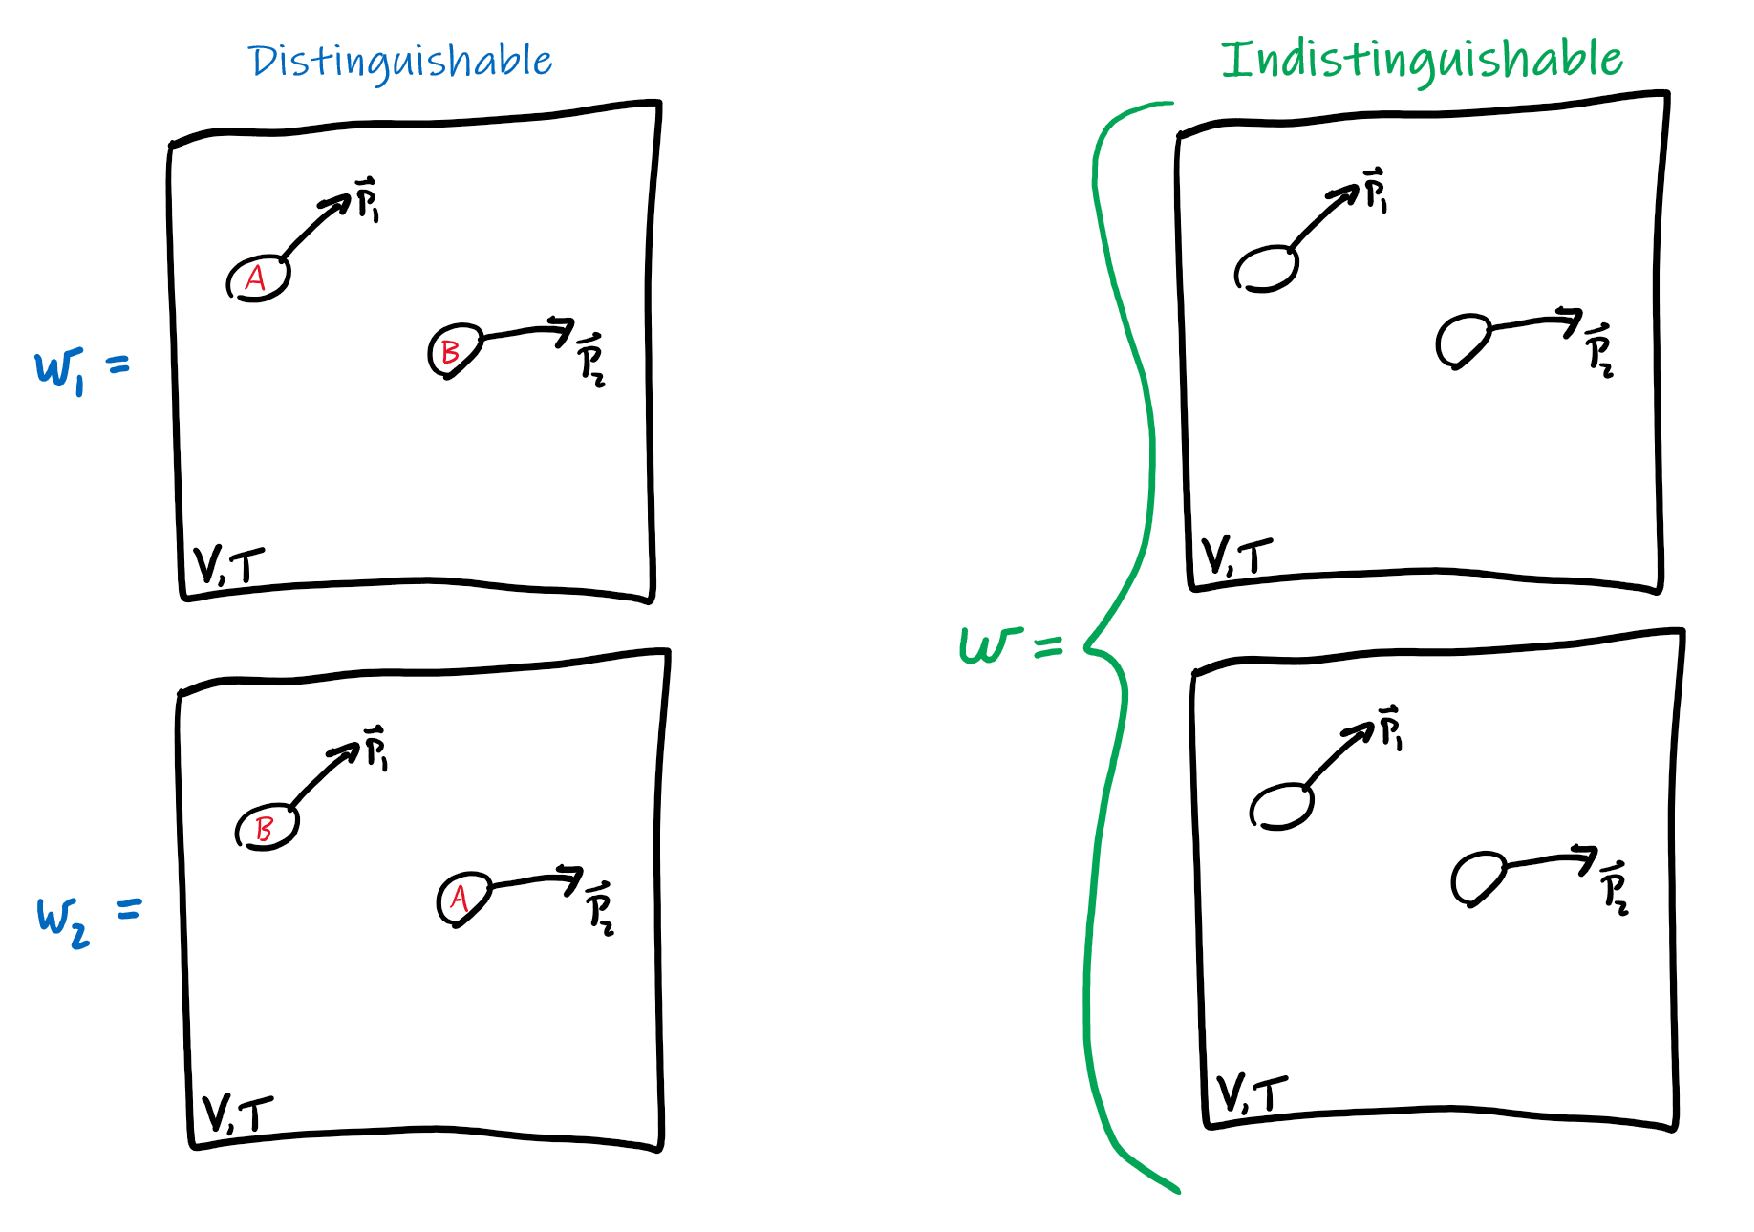
\includegraphics[width=0.7\textwidth]{figs/week04_distinguish.pdf}
\end{center}
If the particles are indistinguishable, no such labeling is possible, and there is only one micro-state for these $\left\{\vec p_1, \vec p_2\right\}$, rather than two.
This factor of $2$ is not accidental, as you can appreciate by counting how many micro-states there are for three distinguishable particles with momenta $\left\{\vec p_1, \vec p_2, \vec p_3\right\}$, compared to the single micro-state for the indistinguishable case:
\begin{mdframed}
  \ \\[100 pt]
\end{mdframed}

In full generality, ideal gases with $N$ distinguishable particles have $N!$ times more micro-states compared to otherwise-identical ideal gases with indistinguishable particles: There are $N$ possible ways to label the particle with momentum $\vec{p}_1$, then $N - 1$ possible labels for $\vec{p}_2$, and so on.
The partition function sums over these micro-states, but depends only on their energies, which are independent of any labeling.
Therefore this factor of $N!$ is the only difference between \eq{eq:ideal_dist} and the partition function $Z_I$ for indistinguishable particles,
\begin{equation}
  \label{eq:ideal_indis}
  Z_I = \frac{1}{N!} \left(\frac{mTL^2}{2\pi\hbar^2}\right)^{3N / 2} = \frac{1}{N!} \left(\frac{L}{\lath}\right)^{3N} = \frac{1}{N!} \left(\frac{V}{\lath^3}\right)^N.
\end{equation}
% ------------------------------------------------------------------



% ------------------------------------------------------------------
\subsection{Internal energy, and entropy}
Now that we have the canonical partition function, let's apply our work from last week to predict the large-scale behaviour of the ideal gas it describes.
Our first targets are the average internal energy $\vev{E}$ and entropy $S$ for the gas, as functions of its fixed temperature $T$, conserved particle number $N$, and the volume $V = L^3$ in which it is placed.
Let's begin with the slightly more complicated case of indistinguishable particles, \eq{eq:ideal_indis}.
Recalling the derivatives in Eqs.~\ref{eq:canon_entropy-F}--\ref{eq:canon_energy-F}, we should keep the temperature dependence explicit in our workings, rather than hidden inside the thermal de~Broglie wavelength $\lath(T)$.

Starting by writing down the Helmholtz free energy,
\begin{equation*}
  F_I = -T \log Z_I = -\frac{3NT}{2}\log\left(\frac{mTL^2}{2\pi\hbar^2}\right) + T \log\left(N!\right),
\end{equation*}
we can quickly extract the internal energy,
\begin{equation*}
  \vev{E}_I = -T^2 \pderiv{}{T}\left(\frac{F_I}{T}\right) = -T^2 \pderiv{}{T}\left(-\frac{3N}{2}\log T + T\mbox{-independent}\right) = \frac{3}{2} NT.
\end{equation*}
This in turn provides the entropy
\begin{equation*}
  S_I = \frac{\vev{E}_I - F_I}{T} = \frac{3}{2} N + \frac{3N}{2}\log\left(\frac{mTL^2}{2\pi\hbar^2}\right) - \log\left(N!\right).
\end{equation*}
We can clean this up by reintroducing the thermal de~Broglie wavelength,
\begin{equation*}
  \frac{3N}{2}\log\left(\frac{mTL^2}{2\pi\hbar^2}\right) = \frac{3N}{2}\log\left(\frac{L^2}{\lath^2}\right) = N\log\left(\frac{V}{\lath^3}\right),
\end{equation*}
and by applying Stirling's formula as we did last week, again neglecting $\cO(\log N)$ terms,
\begin{equation*}
  \log\left(N!\right) = \log\left(N^N e^{-N}\right) + \cO(\log N) \approx -N \log\left(\frac{e}{N}\right).
\end{equation*}
Putting these pieces together,
\begin{equation*}
  S_I = \frac{3}{2} N + N \log\left(\frac{eV}{N\lath^3}\right).
\end{equation*}

\newpage % WARNING: FORMATTING BY HAND
What are the corresponding results for the case of distinguishable particles, where the partition function $Z_D$ is given by \eq{eq:ideal_dist}?
\begin{mdframed}
  $\displaystyle F_D = $ \\[50 pt]
  $\displaystyle \vev{E}_D = $ \\[50 pt]
  $\displaystyle S_D = $ \\[50 pt]
\end{mdframed}
You should find that the energy is insensitive to whether or not we can label the particles:
\begin{equation}
  \label{eq:ideal_energy}
  \vev{E}_D = \vev{E}_I = \frac{3}{2} NT.
\end{equation}
This is in contrast to the spin system we considered last week.\footnote{The origin of this contrast is that each ideal gas micro-state $\om_i$ in the indistinguishable case corresponds to $N!$ micro-states in the distinguishable case, independent of the energy $E_i$.  For the spin system this factor was $\binom{N}{n_+}$ and varied with the energy $E_{n_+}$.}
The entropy, however, does reflect the extra information that distinguishability provides:
\begin{align}
  \label{eq:ideal_entropy}
  S_D & = \frac{3}{2} N + N \log\left(\frac{V}{\lath^3}\right) &
  S_I & = \frac{3}{2} N + N \log\left(\frac{eV}{N\lath^3}\right).
\end{align}
As the temperature approaches absolute zero, $T \to 0$, it appears as though these entropies become infinitely negative---this is a warning sign that our classical assumptions are breaking down and quantum effects would need to be taken into account.
% ------------------------------------------------------------------



% ------------------------------------------------------------------
\subsection{The mixing entropy and the `Gibbs paradox'}
Back in \secref{sec:heat_ex} we considered what would happen if we allowed two micro-canonical ensembles to exchange energy, and then re-isolated them.
We saw that this procedure obeyed the second law of thermodynamics: the entropy never decreased, though we had to be careful to account for all of the entropy after re-isolating the two subsystems.

We can now carry out a similar thought experiment by allowing two canonical ensembles to exchange particles, and then re-separating them.
We demand that both canonical ensembles are in thermodynamic equilibrium with each other, for instance by sharing the same thermal reservoir with temperature $T$.
This procedure is illustrated below, where we simplify the setup by taking the two initial systems to have equal volumes, $V_A = V_B = V$, and numbers of particles, $N_A = N_B = N$.

\begin{center}
  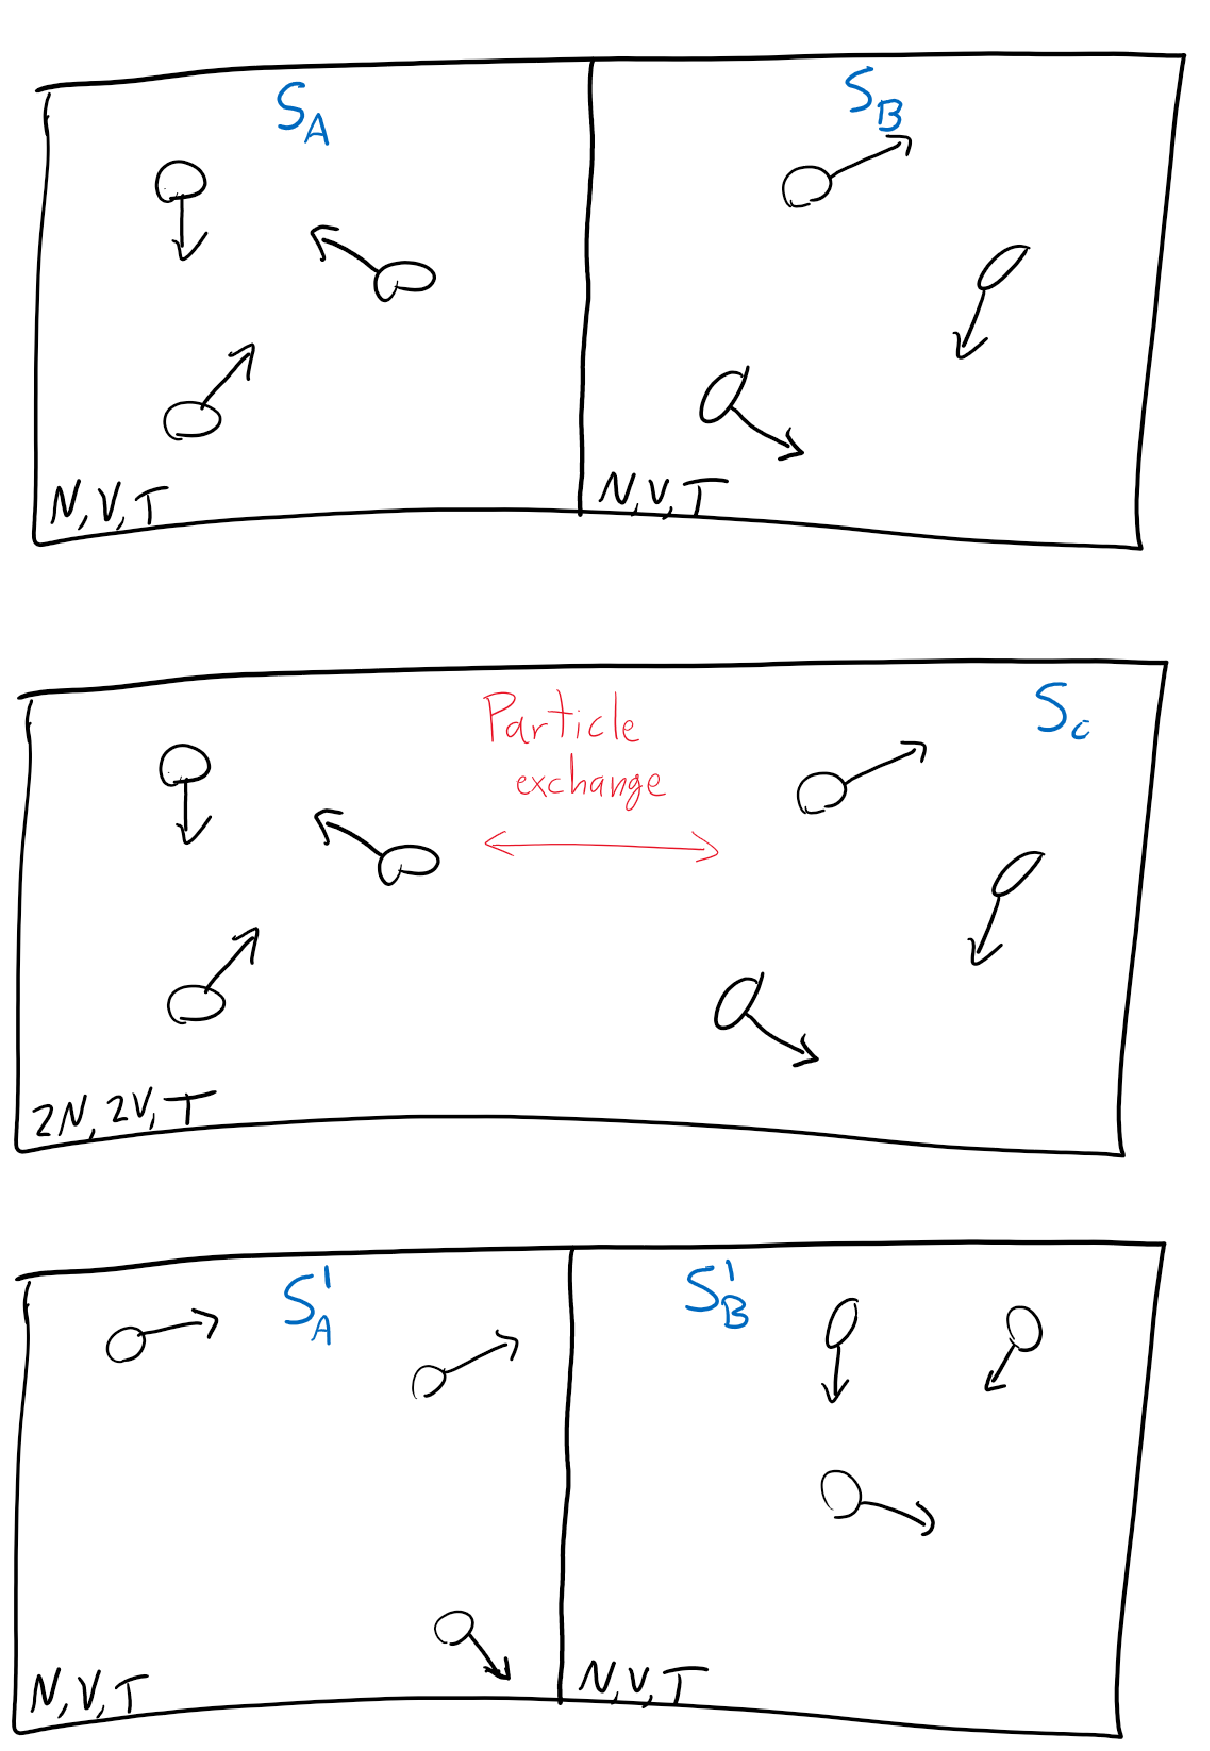
\includegraphics[width=0.7\textwidth]{figs/week04_mixing.pdf}
\end{center}

We can represent the process of combining and then re-separating these systems by writing
\begin{equation*}
  \Om_A + \Om_B \lra \Om_C \lra \Om_A' + \Om_B'.
\end{equation*}
What is the entropy for each of these three stages?
Since the entropies depend on whether or not the particles in the gas are distinguishable from each other, let's first consider the case of \textit{indistinguishable} particles.

\newpage % WARNING: FORMATTING BY HAND
The initial entropy is the sum of the contributions from the two canonical systems, $S_A + S_B$, both of which are the same thanks to our simplification above, and are given by \eq{eq:ideal_entropy}:
\begin{mdframed}
  $\displaystyle S_A + S_B = 2S_I(N, V) = $ \\[50 pt]
\end{mdframed}
To find the entropy $S_C$ of the combined system, we just need to consider what happens when we double the volume and also double the number of particles:
\begin{mdframed}
  $\displaystyle S_C = S_I(2N, 2V) = $ \\[50 pt]
\end{mdframed}
You should find $S_C = S_A + S_B$, which is consistent with the second law of thermodynamics.

Things are more complicated when we re-separate the systems.
Analogously to our considerations in \secref{sec:heat_ex}, we need to sum over all the possible ways of dividing the $2N$ particles between the two re-separated boxes.
If $N_A'$ particles end up in the left box (system $\Om_A'$), then the other system $\Om_B'$ must contain the remaining $N_B' = 2N - N_A'$ particles.
Adding up the entropies,
\begin{align}
  S_A' + S_B' & = \sum_{N_A' = 0}^{2N} \left[\frac{3}{2} N_A' + N_A' \log\left(\frac{eV}{N_A' \lath^3}\right) \right. \cr
              &         \qquad\qquad + \left.\frac{3}{2} (2N - N_A') + (2N - N_A') \log\left(\frac{eV}{(2N - N_A') \lath^3}\right)\right] \label{eq:mixing_full} \\
              & = 3N + 2N \log\left(\frac{eV}{\lath^3}\right) + \sum_{N_A' = 0}^{2N} \log\left[\left(N_A'\right)^{-N_A'} \left(2N - N_A'\right)^{-(2N - N_A')}\right]. \nonumber
\end{align}

Since this is hard to compare with $S_C = S_A + S_B = 3N + 2N \log\left(\frac{eV}{N\lath^3}\right)$, back in the 1870s J.\ Willard Gibbs suggested considering only the case $N_A' = N_B' = N$.
This is justified for large numbers of particles, $N \gg 1$, because there are \textit{very} many ways of choosing $N$ out of the total $2N$ particles to end up in $\Om_A'$,
\begin{equation}
  \label{eq:mixing_factorial}
  \binom{2N}{N} = \frac{(2N)!}{N! \; N!} \gg 1,
\end{equation}
compared to (for example) the single way of choosing $N_A' = 0$.
This is the case drawn in the illustration above, and with this approximation we have $\Om_A' = \Om_A$ and $\Om_B' = \Om_B$.
Therefore the final entropy is simply $S_A' + S_B' = S_A + S_B$ and the second law of thermodynamics is satisfied:
\begin{equation*}
  S_A' + S_B' = S_C = S_A + S_B.
\end{equation*}
This is what we would expect from everyday experience: opening a door between two identical rooms doesn't lead to any observable effects, nor does reversing that process by closing the door.

Something interesting happens when we repeat the same procedure for the case of \textit{distinguishable} particles, using our result for $S_D(N, V)$ in \eq{eq:ideal_entropy}.
If we consider the difference between the combined entropy $S_C$ and the initial entropy $S_A + S_B$,
\begin{align}
  \De S_{\mathrm{mix}} & = S_C - (S_A + S_B) = S_D(2N, 2V) - 2S_D(N, V) \cr
                       & = 3N + 2N \log\left(\frac{2V}{\lath^3}\right) - \left[3N + 2N \log\left(\frac{V}{\lath^3}\right)\right] = 2N\log 2 > 0,
\end{align}
we find that the entropy increases upon combining the two initial systems.
This $\De S_{\mathrm{mix}} > 0$ is known as the \textbf{mixing entropy}.

This result $S_C > S_A + S_B$ is what we would expect from the second law of thermodynamics.
However, repeating the argument above that we can approximate $\Om_A' = \Om_A$ and $\Om_B' = \Om_B$ would then imply $S_A' + S_B' < S_C$, indicating a \textit{decrease} in the entropy by $\De S_{\mathrm{mix}}$ and an apparent violation of the second law of thermodynamics.
This is known as the `Gibbs paradox', though Gibbs himself explained how the paradox is avoided.

Because the particles are now distinguishable, $N_A' = N_A$ is no longer sufficient to establish $\Om_A' = \Om_A$.
We need to specify not only that the total number of particles is the same, but also that the same distinguishable particles initially in $\Om_A$ also end up in the final $\Om_A'$.
For example, if we start with particles $\left\{A, B, C\right\}$ in system $\Om_A$ with $\left\{D, E, F\right\}$ in $\Om_B$, then there is only a single way of ending up with $\left\{A, B, C\right\}$ in $\Om_A'$ and $\left\{D, E, F\right\}$ in $\Om_B$, not the factorially large number (\eq{eq:mixing_factorial}) that let us justify Gibbs's approximation. % TODO: Could mention un-mixing coffee and cream, though those are interacting fluids rather than ideal gases...
Therefore we have to sum over all the possible ways of distributing all $2N$ distinct particles into the re-separated systems, analogously to \eq{eq:mixing_full}.
It's not illuminating to grind through that calculation; we can be content to observe that the `Gibbs paradox' does not arise and the second law of thermodynamics remains valid.

We can also observe another example of physical effects that differ depending only on the intrinsic information content of the system---whether or not the particles in an ideal gas can be distinguished from each other in principle.
While mixing gases of distinguishable particles introduces a positive mixing entropy, for gases of indistinguishable particles there is no change in entropy when we let two subsystems mix, or when we reverse that process and re-separate them.
% ------------------------------------------------------------------



% ------------------------------------------------------------------
\subsection{Pressure and the equation of state}

\TODO{Adiabaticity and constant-entropy condition...}

\TODO{Being written...}
% ------------------------------------------------------------------
